\documentclass[11pt]{report}
\usepackage{hyperref} 
\usepackage[official]{eurosym}
\usepackage{footnote}
\usepackage{graphicx}
\newcommand\footnoteref[1]{\protected@xdef\@thefnmark{\ref{#1}}\@footnotemark}
%Gummi|065|=)

\begin{document}

\begin{centering}
\Large Welcome to Data Insights!\\
\end{centering}
\vspace{2cm}

Hi! Welcome to Data Insights! My name's Evan, and I started with this company 2 months ago. So I'm also pretty new (at the time of writing this). Over the past 2 months, I have learned a lot of things from a lot of different people. So I thought it could be good to put all that information in one single place. So here it is! I hope it helps you getting started with a really cool new company (ours).\\

\noindent\textbf{At the end of this document you'll find a step-by-step list of what you need to do. So go there if you're feeling like a lost soul :)}

\tableofcontents

%#########################################################################################################
\chapter{Before you Show Up}
%#########################################################################################################

\section{Tech Stuff!}
\label{TechStuff}
Firstly, it's important to get you a new phone and laptop\footnote{If there is an unclaimed laptop or phone which is under 3 years old, it is possible that you are asked to use that one until it is 3 years old, at which point you will be given a new one. The Laptop/Phone will, in that case, be wiped, so it will be as good as new :)}. Even if you already have them, we prefer if you have a company one. Please let us know ASAP which ones you want, so we can order them and have them ready for your arrival.

\subsection{Laptop}
There are two options for the laptop. You can choose either:\\
$\rightarrow$ Dell XPS 15\footnote{Running Windows 10. You are free to install Linux, however we prefer you maintain Windows in a partition. I (Evan) can help you set this up if you'd like.}{\tiny (\href{https://www.dell.com/de-de/shop/laptops-2-in-1-pcs/xps-15/spd/xps-15-9570-laptop/cnx97004}{https://www.dell.com/de-de/shop/laptops-2-in-1-pcs/xps-15/spd/xps-15-9570-laptop/cnx97004})}\\
or:\\
$\rightarrow$ Mac Book Pro 15'', 16GB RAM {\tiny \href{https://www.apple.com/shop/buy-mac/macbook-pro/15-inch-space-gray-2.6ghz-6-core-512gb}{https://www.apple.com/shop/buy-mac/macbook-pro/15-inch-space-gray-2.6ghz-6-core-512gb}}\\
Both come with a 3 year warranty. For purposes of standardising software, we only allow the work laptop to be one of these two choices. Also, {\bf please let us know which style of keyboard you want!}

\subsection{Phone}
The budget for the phone will be 300 \euro, however for iPhones we will allow up to 380 \euro. You are welcome to request a more expensive phone and cover the difference. The included plan will be through Telekom, with 2 Gb of data monthly, and unlimited calls and texts within Germany.

\section{Personal Information} \label{PersonalInformation}
In addition to the above information, you will need to provide the following:
\begin{itemize}
\item Full Name (as it appears on your passport)
\item Date of Birth
\item City of Birth
\item If you are not German, copy of your work permit, or EU passport.
\end{itemize}
Please send this all ASAP!




%#########################################################################################################
\chapter{Your First Day! :D}
%#########################################################################################################

Oh gosh! Today's the day! I hope you packed a healthy lunch and wore your lucky underwear. So here's what's happening:

\section{Paperwork}
\label{paperwork}
Yeah, so it's not the most fun thing to start with, but the HR will give you a paper to fill out. It might take a while, as you will need your bank info and insurance number, but just keep it in mind as you being your document collecting journey.

\section{Introductory E-Mail}
\label{Email}
By now you've probably already given all your info to the HR. You should now get an e-mail address. This will have the format \emph{name}@datainsights.de. You will need this e-mail for a lot of the tasks below, so I figured I would mention it now. 

When you get the e-mail address, we ask that you send an e-mail to all.datainsights@datainsights.de to introduce yourself. Please include a little info about your background, as well as a picture so we all know who you are.

Even if you don't have the e-mail yet, it could be a good idea to keep reading. Lots of neat stuff to know!

\section{The Jungle}
Data Insights in run out of a really awesome space, affectionately known as `The Jungle', located near Goetheplatz UBahn station in central Munich. We have beanbag chairs, a kicker\footnote{`Foosball' for those from North America.} table, and a fridge always stocked with candy and beers. What else do you need?
\subsection{Wifi}
\label{wifi}
Username: Data Insights GmbH\\
Password: datainsightsjungle!
\subsection{The Key}
\label{TheKey}
The office uses a digital lock. To open the door you must first download an app called Nuki (on your company phone, so you'll have to wait for it to arrive). Then ask the HR to send you a Nuki invitation e-mail. Once you have that, activate your phone's bluetooth. When you are near the door, open the app, click on `Jungle', and you will see the option to open the door (if it's not working, pull the door towards you slightly while clicking unlock). If you are the last person to leave the office, you can also follow the same procedure to lock the door.

\subsection{Food}
Oh, and there is also lots of food around the office. The fridge is stocked with soda and beer, there is tea and coffee, and there are usually candies and fruits on the table. Help yourself (within reason), and if you drink a soda or beer, please go downstairs to drop the bottles in the recycling, and then bring an unopened bottle back up to put in the fridge and replace the one you drank.

\subsection{Etiquette}
Even if it's called the Jungle, we don't want to be animals. So, a few little notes to keep in mind:
\begin{itemize}
\item Clean up after yourselves (keep the sink area clean, put dishes in the dishwasher, follow the rules posted in the bathroom and on the fridge).
\item Before leaving, tidy up your desk space so others can use it (especially on Fridays, as a cleaner comes).
\item If you are the last person leaving the office, make sure the windows are closed, the lights are off, and the dishwasher has been turned on.
\end{itemize}
We often have customers and partners coming to the office, so we don't want to scare them off by letting them know that we're slobs (not that we actually are...\emph{cough}...).

\section{The Perks}
Besides the laptop and phone, there are lots of neat things that come with working at Data Insights. Let's go through some of them!

\subsection{Lots of Training}
\label{Training}
If you are a junior, we provide up to 5,000 \euro{} for training relevent to your domain (workshops, technical training, online certification, etc.). For seniors, the budget is 3,000 \euro{}. This training can be anywhere (within reason), and can last up to 10 days\footnote{\label{note1} Assuming the training takes place during the regular workday. Evening and weekend courses don't count towards this total.}. In the case of German courses, we allow up to 30 days$^{\textrm{\scriptsize \ref{note1}}}$ of courses, if necessary. Course materials (books, etc.) can also be reimbursed.

\subsection{30 Days Vacation}
\label{Vacation}
Data Insights offers 30 days of paid vacation per year (on top of holidays, obviously). To keep track of who is taking holidays, and their specific dates, Data Insights uses a program called \underline{TimeButler}, which you can find here: \href{https://timebutler.de/do}{https://timebutler.de/do}.

You will need to talk to the HR about opening a TimeButler\footnote{We are soon switching to a new interface called Zoho, so keep an eye on that...} account using your company e-mail. Be sure to declare any holidays you take in advance using the interface, and also discuss with your company if you are working on a project.

It is important that you take your days each year! The German government gets mad at us if they think we are overworking our employees, and they look into how much vacation we are taking. So plan accordingly.

\subsection{Social Days}
\label{social}
In addition to the 30 days of vacation, Data Insights also insists on 3 paid days of social work each year. On these days you must engage in any form of social work, anywhere in the world. The definition is very broad: in the past our employees have undertaken local projects such as cleaning up garbage and distributing food, as well as international projects such as teaching children in India and providing clothes in Mexico. The sky is the limit! We also appreciate any photos or videos you can provide of your work, so we can add it to the website: \href{https://datainsights.de/social-days/}{https://datainsights.de/social-days/}

\subsection{Urban Sports Club Membership}
\label{Sports}
Another great perk is the free Urban Sports Club Membership! This gives you access to lots of sports facilities and gyms all around Munich (Germany, and some of Europe), for nearly any sport you can imagine. To sign up, start here (the link is a bit long, sorry):

\noindent \href{https://urbansportsclub.com/en/datainsights?utm_source=Onboarding+CS+-+DE&utm_campaign=432b2f55f5-Data+Insights_muc_onboarding_winter&utm_medium=email&utm_term=0_8eb1bd3f3b-432b2f55f5-110213073}{\tiny https://urbansportsclub.com/en/datainsights?utm\_source=Onboarding+CS+-+DE\&utm\_campaign=432b2f55f5-Data+Insights\_muc\_onboarding\_winter\&utm\_medium=email\&utm\_term=0\_8eb1bd3f3b-432b2f55f5-110213073}

When asked to choose the plan, choose the `M PRO' option\footnote{You can also choose the L PRO or XL PRO options if you wish. You receive a discounted rate for applying through Data Insights, however you will still have to pay.}. Then follow the sign-up steps (use your company e-mail).

When you have downloaded the Urban Sports Club app, you are ready. On the app you will find a map of all the locations included (or you can search by sport). In general, when you go to a venue you simply scan a QR code via the app, and you can go in for free. Some venues without a QR code may require you to take a picture of your receipt and send it to cashback@urbansportsclub.com. Then they will send you a reimbursement.

One other neat thing. If you have a `someone special' in your life, then they can also qualify for a reduced rate (I think it's 30\% off) if they register through this page:
\href{https://urbansportsclub.com/en/datainsights_familyandfriends}{\tiny https://urbansportsclub.com/en/datainsights\_familyandfriends}.


\subsection{Trips and Events and Stuff}
And finally, there are lots of other neat things to look forward to! Here's a non-exhaustive list:
\begin{itemize}
\item Paid monthly dinners at great restaurants around Munich (usually the last friday of the month).
\item A wild Summer Party!
\item An even wilder overnight Winter Party!
\item Oktoberfest table
\item Monthly `Data Talks', in which we all get together to discuss data stuff and eat pizza.
\item The possibility to go represent Data Talks at conferences and hiring events around Europe.
\end{itemize}

\section{Management 3.0}
One of the neat things about Data Insights is that we operate on a concept known as `Management 3.0'. The idea is that there is no `boss' in the company. Individuals are responsible for everything: overseeing and managing internal projects, maintaining the workspace, setting and achieving profit margins, and even the hiring process (hence why I'm writing this now).

To give you an example, about a month ago it was decided we needed a technical test for certain employees (maybe you were one of them?). So we all got together, including myself (and I'd only been around for a few weeks), and we devised and designed the test over the course of a few weeks. The company founders, who were quite busy, had no say in the test. It was entirely us.

The model is quite empowering, but it can also be quite a bit of work. The following is what you need to know to keep the company running smoothly, including the tools we use to achieve this.

\subsection{Slack}
\label{Slack}
\href{https://datainsightsde.slack.com}{https://datainsightsde.slack.com}\\

Slack is a chat interface we use to communicate amongst ourselves. Ask the HR to add you to Slack, as well as to the various sub-groups within the Data Insights slack channel (fun-sports, random, general, etc.). You will figure out the interface pretty fast. One other important thing: Every Friday in the General thread there is a `company update post'. Be sure to write a quick summary of what you are up to each week.

\subsection{Perdoo}
\label{Perdoo}
\href{https://web.perdoo.com}{https://web.perdoo.com}\\

Perdoo is an online system that helps us with task organisation in the Management 3.0 framework. It follows a principle known as `OKR': Objective, Key Result. For each task, you define a qualitative \underline{Objective} (e.g. `New employees need to be better trained') and a few quantitative \underline{Key Results} (e.g. `There should be a single document that allows new employees to be introduced to the company in just an hour'). Lastly, under the Key Results we add \underline{Initiatives}, which are actions that we can take to achieve each result. Perdoo is meant to allow for more transparency with respect to business goals, helps us focus on things which truly matter, and helps us visualise our progress.

You will want to get Marketing to make you a Perdoo account, and then access the training by doing the following:
\begin{enumerate}
\item Go to this link: \href{https://datainsights-perdooacademy.talentlms.com/}{https://datainsights-perdooacademy.talentlms.com/}
\item Click on `Create Account'.
\item Once you're logged in, the relevant courses should be visible.
\end{enumerate}

\begin{figure}[!htb]
        \center{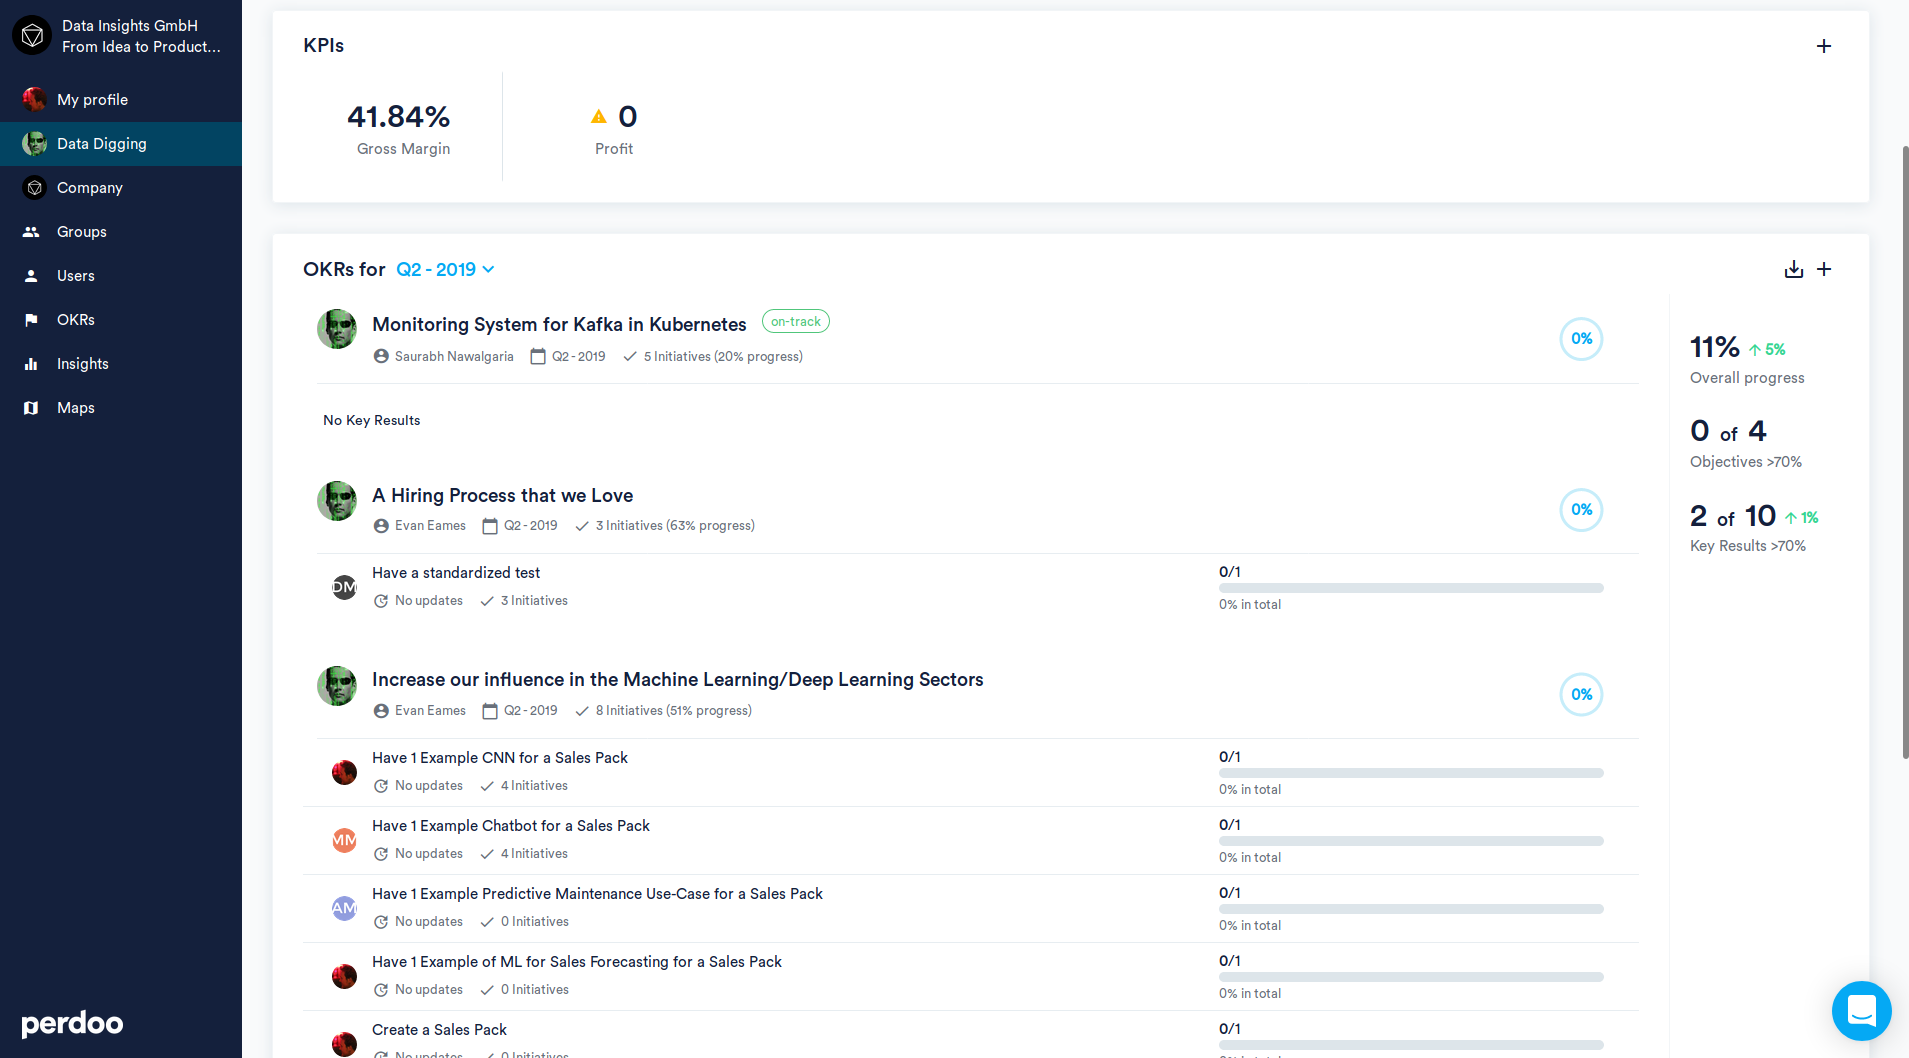
\includegraphics[width=\textwidth]{perdoo.png}}
       \caption{\label{fig:perdoo} The DDT team perdoo board.}
\end{figure}

In figure \ref{fig:perdoo} you will see an example of the DDT Perdoo board. When you are thinking of starting a new task, take a moment to think of which of the company Objectives, or which Key Result, it will fall under. Once you've done that, add the task as a Key Result (if it directly supports and objective), or an Initiative (if it is a step towards achieving a Key Result. As you continue to work on various tasks, be sure to regularly update their status in Perdoo.

\underline{Note:} Perdoo was introduced in April 2019. Before this we were using another system called `Scrum', which was run out of an interface called `Jira'. I've still included a description of this previous interface below (see `Jira' under section \ref{Jira}). Even if we are no longer using Scrum, some of the tasks are still listed in the Scrum backlog, so if you're looking for something to do, it could be good to start there, and then add it to Perdoo when you begin.

\subsection{Atlassian}
\label{Atlassian}
\href{https://datainsights.atlassian.net}{https://datainsights.atlassian.net}\\

Compared to Slack and Perdoo, Atlassian takes a bit more getting used to (I'm still figuring it out). It is a big multi-purpose website which manages lots of things going on in the company. Ask HR to add you to Atlassian. On the bottom left corner you will see a grid-icon between the Bell icon and the Question mark icon. Click this to switch between the two sub-sections of Atlassian: Confluence and Jira.

\subsubsection{Confluence}
Confluence allows us to post and share files. Note that it's divided into teams (DDT\footnote{Data Digging Team}, Ab Initio, Company Organisation, etc.). You can click on the Spaces Folder icon to see all the spaces. To give you an example, in the `Administrative Space' you can find an alphabetical list of topics that are relevant to the company's functioning: \href{https://datainsights.atlassian.net/wiki/spaces/AS}{https://datainsights.atlassian.net/wiki/spaces/AS}. When you need documentation on any of the software we use, or the company in general, this could be a good place to start.

\subsubsection{Jira}
\label{Jira}
\textbf{As of April, 2019, we have begun to switch from Jira/Scrum (outlined here) to the Perdoo system, described above. Jira is still operating, however, so here's an outline anyway.}

The second aspect of Atlassian is called Jira. This interface is essential to making Management 3.0 work. When you go to Jira, you will see a calendar with a number of orange squares. Each one of these is a task that must be completed. You can click on them and see a description of the task. By clicking the `Projects' folder on the left, and then choosing `Data Insights Organisation' you can see what is called the \emph{Sprint Board} (see figure \ref{fig:Sprint Board}).

\begin{figure}[!htb]
        \center{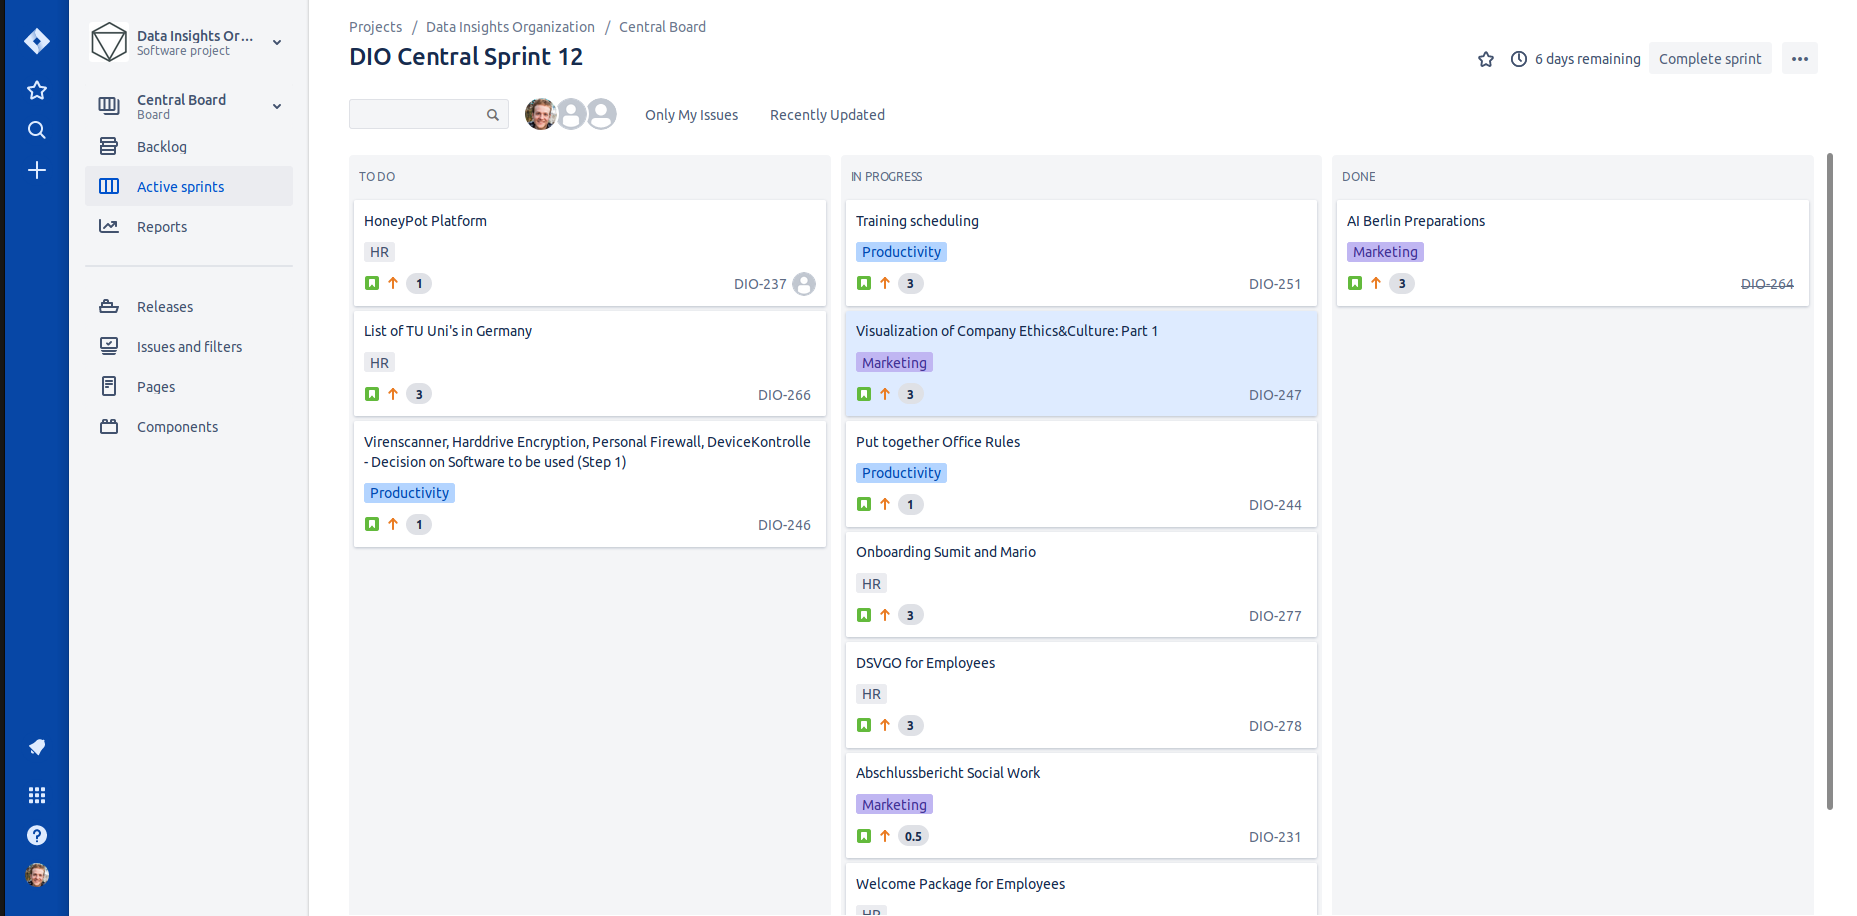
\includegraphics[width=\textwidth]{SprintBoard.png}}
       \caption{\label{fig:Sprint Board} An example of a sprint board (from Jira).}
\end{figure}
Here's how it works. Firstly, on the left, you will see a few options. One is called \emph{backlog}. Here, anyone can go and write-up a task\footnote{Specifically, an internal task, which doesn't have to do with external projects/companies.} that they think needs to be done. Every 4 weeks, the employees get together to define a \emph{sprint} for the next month. They choose some tasks from the backlog, and put them on the current \emph{sprint} (in the `To Do' section). If you look again at figure \ref{fig:Sprint Board}, you will see that some tasks have been switched to the `In Progress' column, and one has been `Done'. This helps us keep track of the tasks that need to be finished, and whether they have been started. At the end of the month, unfinished tasks are moved to the next \emph{sprint}, and new tasks are added from the backlog. By the way: This system of monthly \emph{sprints} is called \textbf{scrum}.

So, if you happen to be without a project (or, as we say here, `on the bench'), then go look at the sprint board to see if there is anything you can potentially help out with. While working on a task, add some comments to the task so people know how it is progressing. If you are super busy on a project, and have no time for internal tasks, don't worry!

Oh, one last comment: On the left hand panel you can also switch between the sprint boards for different groups within Data Insights (Ab Initio, Central, and DDT). Check the one that applies to you!

\subsection{Kanban}
There is discussion of also using a system called `Kanban' alongside Perdoo. Kanban is a ultra-simple task management method, in which you simply list tasks as being `Not started', `In progress', or `Complete'. There is really nothing else to it. We will be seeing how we do with Perdoo, and then maybe we won't actually need it. Stay tuned! I figured I should just mention it here anyway.

\subsection{Finances}
Data Insights makes all of its financial information fully transparent. That means that any employee can see the full list of profits, losses, expenditures, and outlook for a given month or quarter. In addition, every quarter there is a meeting to assess the current financial situation, and prepare an outlook for the coming quarter. This is a good time to figure out who will be on projects in the coming month, and who will be on the bench, or on vacation.

The finance documentation can be found here:\\
\href{https://datainsightsde.sharepoint.com/sites/all/Freigegebene\%20Dokumente/Forms/AllItems.aspx}{\scriptsize https://datainsightsde.sharepoint.com/sites/all/Freigegebene\%20Dokumente/Forms/AllItems.aspx}\\
Click on your team (DDT, AbInitio, HR, etc.) and then click the P\&L (profit \& loss) directory. By the way, I should mention that the above link is our company \textbf{sharepoint}. It's here that we store all the crucial documents related to our Company's functioning (as opposed to Confluence, which is more general).

\subsection{So many tools!}
How about a quick rundown of all these tools?
\begin{itemize}
\item \textbf{Slack} -- Chatting, weekly company updates, etc. Check it daily.
\item \textbf{Perdoo} -- Task management. What are you doing? Why are you doing it? Update as you do stuff.
\item \textbf{Atlassian} -- A web interface which contains:
\begin{itemize}
\item \textbf{Confluence} -- Storage of general documents
\item \textbf{Jira} -- Contains \textbf{Scrum}, our old task management system (now replaced by Perdoo). There is still a backlog of tasks to-be-done here that could still be useful.
\end{itemize}
\item \textbf{Sharepoint} -- Storage of crucial documents, such as the Profit \& Loss information.
\item \textbf{TimeButler}* -- Where we register and track our vacation.
\item \textbf{Papierkram}* -- Where we register our days on a project (described in section \ref{when you're needed} below)
\end{itemize}
{\scriptsize * These will soon be combined into a single system called Zoho.}

\section{Projects}
\label{Projects}
Okay, so we're almost through this! The last little bit is simply explaining projects. This is when you get paired with a company to do some work for them.

\subsection{While waiting}
While you're waiting to be assigned to a project, you should focus on the following:
\begin{itemize}
\item Do some of the internal tasks listed on Perdoo (section \ref{Perdoo}), or you can also tackle some in the Scrum backlog (section \ref{Jira}).
\item Talk to people to see what training may be useful for you (Cloudera\footnote{Talk to Saurabh about using his account, but only if you need one.}, Coursera, AWS\footnote{Talk to Socrates about creating an account, but only if you need one.}, etc.).
\item Take care of those social days! (section \ref{social})
\item If it doesn't look like there will be a project in the immediate future, perhaps take a nice vacation!
\href{https://www.google.com/flights}{https://www.google.com/flights}
\end{itemize}

\subsection{When you're needed}
\label{when you're needed}
Eventually you will be asked to potentially join a project. You will likely discuss with the company to see if you have the competencies they are looking for. \textbf{Note: Don't mention to one company if you have other potential companies who you are also in discussion with.} This is important if one project falls through (you will still have another).

If they agree on the project, you will have to discuss how often you will be expected to be `on-site' (at the company). Some companies don't mind their data scientists working from a distance, while others prefer them to be `on-site'. Then some others prefer for them to be there only a few times per week\footnote{Also, if you have to be in Berlin on a Monday, for example, it is usually understood that Monday will include your travel time (leaving from Munich Monday morning by train, as opposed to Sunday night).}.

Regardless of whether or not you have to travel for work, you still need to ask HR about giving you a \underline{Papierkram} account\footnote{This will also become Zoho soon.}:\\
\href{https://datainsights.papierkram.de/login}{https://datainsights.papierkram.de/login}\\
You will use this when you log how many days you work for a company.

\subsubsection{Travel}
If you need to travel for your work:
\begin{enumerate}
\item First create a \underline{Bahn Business} account (you can ask HR for help with this one):\\
\href{https://www.bahn.de/p/view/bahnbusiness/index.shtml}{https://www.bahn.de/p/view/bahnbusiness/index.shtml}
\item And finally, fill out an expense report after your trips:\\
\href{https://datainsights.atlassian.net/wiki/spaces/AS/pages/33296607/Expenses}{https://datainsights.atlassian.net/wiki/spaces/AS/pages/33296607/Expenses}
\end{enumerate}

When you travel, the base base budget is 150 \euro{}. There is an additional daily allowance for projects where you have to be out of Munich. This will depend on the country, but for Germany the allowance is 12 \euro{} for a project that requires you to be away from Munich for time $t$ where $8 \leq t \leq 24$, and then 24 \euro{} per day for anything greater. Talk to the HR to get the values for other countries.

Lastly, you have two options for paying. You can either pay for transport and hotels yourself, file the expense report, and then receive the money back at the end of the month. Or you can talk to the BackOffice\footnote{A funny German term for `administration'.} about booking transport and hotels directly. The daily allowance must be refunded via the expense report form.

\subsection{Aftermath}
When you finish your project, it's also important to add a description of your project to your Data Insights CV. Then rinse and repeat!

\section{Still Need Help?}
\label{help}
If at any point you need some help regarding a project, training, or general aspects of the company, here are two resources to help.

\subsection{Skill Matrix}
We try to maintain a skill matrix, which you can query if you are looking for someone with a certain skill. Right now it's hosted here:\\
\href{https://trinket.io/python/7cf239657b}{https://trinket.io/python/7cf239657b}\\
As an example, if you wanted to discuss with someone who knows Hadoop, you type `Hadoop'. You will then be asked if you want a `wizard' (somebody who is really good at something). You can choose yes or no, and will be given a list of people who match your criteria. It doesn't just need to be computer related stuff. You can also search things like `marketing', `hr', `profit and loss', etc. The skill matrix is regularly updated from a master-backup hosted on my google drive:\\
\href{https://docs.google.com/document/d/1jPwwEUulaowHr-lCvzkNiqXkhgfgvQWJrkaa0T4ZKkA/edit?usp=sharing}{\scriptsize https://docs.google.com/document/d/1jPwwEUulaowHr-lCvzkNiqXkhgfgvQWJrkaa0T4ZKkA}\\
Feel free to update it and add your own skills as you learn new stuff.

\subsection{Buddy System}
You are supposed to be paired with a senior `buddy' when you arrive at data insights. This is someone you can go to if you are unsure about something, or are just feeling a little lost for direction in general. In \emph{theory} you should be paired with someone immediately, but it will depend on who is not on a project, and which group you are in. If you aren't assigned a buddy, come to me (Evan) and we'll find you one.

\section{Odds \& Ends}
That's about everything you should have to know to get started. The rest should be obvious:
\begin{itemize}
\item There are no fixed working hours while you're on the bench, but try arrive and leave at a reasonable hour.
\item Let your team know via Slack if you are sick, or if, for whatever reason, you need to work from home for part of the day.
\item Dress appropriately when working at companies.
\item Read the Company Rules (on Confluence).
\item If you experience any form of harassment, immediately make it known to the HR.
\end{itemize}

%###########################################################################################################
\chapter{Settling in M\"unchen}
%###########################################################################################################
So, after I made this document, the HR people liked it so much that they asked me to add a section explaining how to settle in Munich. So here it is.

\section{Visa}
If you're here on an EU passport, like me\footnote{At least until Brexit...}, you're good to go, no visa required.

Otherwise you'll need a work visa. This is a pretty heavy topic, and will depend on your country of origin. To get started, check the website of the nearest German Consulate or Embassy. Maybe also give them a call. You'll probably have to bring a copy of the work contract and passport to show them, among other documents.

Usually you will get a short-term work visa, and when you come to Germany you will have to register to get a long-term work visa. You will likely also quality for a \textbf{Blue Card}, which allows you to live and work in Germany for up to 4 years, and after two years you can apply for Permanent Residency. That's about all the info I have for this.

\section{Banks}
Dang, another complicated one. I use ING and have been quite happy with them. N26 is also supposed to be good.

\section{Public Transport}

Munich's public transport system consists of buses, trams, metros (U-Bahn\footnote{Untergrundbahn -- Underground Railway}), and trains (S-Bahn\footnote{Stadtschnellbahn -- Fast City Railway}). The ticket prices are based on a ring-system you can see here:\\ \href{https://www.mvv-muenchen.de/fileadmin/mediapool/03-Plaene_Bahnhoefe/Tarifplaene/MVV_Tarifplan_Gesamtnetz.pdf}{\tiny www.mvv-muenchen.de/fileadmin/mediapool/03-Plaene\_Bahnhoefe/Tarifplaene/MVV\_Tarifplan\_Gesamtnetz.pdf}
If you want to buy a monthly pass, find which ring you live in, go to a terminal, choose `IsarCard', then select `Von Ring 1 bis \_\_\_\_'. If you ever want to travel to rings beyond the range you selected (to get to the airport for example), you will have to buy a separate ticket. Oh, and there is also an `IsarCard9Uhr', which is much cheaper, but doesn't let you travel between 6~am and 9~am on weekdays. Here's the price breakdown (rounded to the nearest euro):\\

\noindent For the IsarCard:\\
{\tiny \noindent
\begin{tabular}{c||c|c|c|c|c|c|c|c|c|c|c|c|c|c|c|c|}
1 to: & 2 & 3 & 4 & 5 & 6 & 7 & 8 & 9 & 10 & 11 & 12 & 13 & 14 & 15 & 16\\
\hline
\euro{} & 55 & 67 & 79 & 90 & 104 & 117 & 128 & 141 & 153 & 163 & 175 & 188 & 201 & 213 & 226\\
\end{tabular}
}\\

\noindent For the IsarCard9Uhr:\\
{\tiny \noindent
\begin{tabular}{c||c|c|c|}
Rings: & 1 - 4  &  5 -  16 & 1 - 16 \\
\hline
\euro{} & 60 & 60 & 81 \\
\end{tabular}
}\\

You can also buy a 1 year ticket online, and end up saving quite a bit of money. The info for that is here:\\
\href{https://www.mvv-muenchen.de/en/tickets-and-fares/online-und-handyticket/index.html}{\scriptsize https://www.mvv-muenchen.de/en/tickets-and-fares/online-und-handyticket/index.html}\\

Whichever pass you get, it lets you ride on anything (bus/tram/U-Bahn/S-Bahn), as long as you stay in the correct rings. If you need a single ticket, don't forget to validate it before riding the train (there are these little blue boxes on the platforms that you put your ticket in, and it stamps it). Munich ticket controllers dress in normal clothing and will suddenly appear out of nowhere, and they are really scary, so it's best to always keep your ticket on you.

Anyway, all the info is here: \href{https://www.mvv-muenchen.de/en/}{https://www.mvv-muenchen.de/en/}\\

But really you should be biking around to save the planet. Munich has excellent bike-paths, and a bike-share system too (which you can register for here: \href{https://www.callabike-interaktiv.de/en/register?}{https://www.callabike-interaktiv.de/en/register?}).

\section{Insurance}
You also have to register for an insurance provider. I think TK is pretty good. You can register here: \href{https://www.tk.de/en}{https://www.tk.de/en}, and they'll send you a card. With that, you have access to free health care and dental care. Yay socialism!

\section{Finding a Flat}
This is also a huge thing I can't summarize because my gf found our flat. So hopefully Sasha or somebody will write this.

\subsection{Registration}
I can tell you, however, that once you find a place your landlord will provide you with a document that you must bring to the nearest `Rathaus' for the `Anmeldung' (registration). Bring your passport too. They will give you a paper proving you're registered in Germany, then never ever lose that paper.

%###########################################################################################################
\chapter{Final List}
%###########################################################################################################
Okay, deep breath. So, one more time let's run through all the really important stuff you are going to need to do.\\

\noindent \textbf{Before you show up:}
\begin{enumerate}
\item Send laptop/phone/keyboard preferences (section \ref{TechStuff}), as well as personal info (section \ref{PersonalInformation}) to the HR.
\item Get your personal Data Insights e-mail address (section \ref{Email}).\\

\hspace{-0.95cm}\textbf{Once you arrive:}
\item Get on the wifi (section \ref{wifi}).
\item Send an introductory e-mail to the team (section \ref{Email}).
\item If you haven't already, switch your CV to the Data Insights format (and possibly also Reply format if needed). Ask HR for the template.
\item Register for Slack via the HR (section \ref{Slack}).
\item Register for Atlassian via the HR (section \ref{Atlassian}).
\item Register for Perdoo via the HR, and complete the training (section \ref{Perdoo}).
\item Register for TimeButler via the HR (section \ref{Vacation}).
\item Download Nuki on your company phone, and practise opening the door (section \ref{TheKey}).
\item Consider any training that may be useful for your future projects (section \ref{Training}).
\item Sign up for your Urban Sports Club Membership (section \ref{Sports}).
\item If you've done all that, then follow the steps in section \ref{Projects}.
\item And if, after all this, you are still feeling lost, take a deep breath and refer to section \ref{help}.
\item Make the most of life, find your own personal fulfilment, make those around you happy, treat the planet well, pass on your knowledge to the next generation, and die at an old age with a grin on your face.
\end{enumerate}
\vspace{1cm}
\begin{center}
:)
\end{center}
\end{document}